\section{Scattering across the light-vector scale}\label{sec:scattering}

Let $\mathcal M_{\rm YM}$ be the tree amplitude for
$\phi\chi\to\phi\chi$, where $\phi,\chi$ are the canonical massless
scalars with internal states $\mathsf u,\mathsf v$. It is defined by the
leading ten-dimensional action \eqref{eq:YMaction} on
$\mathbb R^{1,5}\times(S,L^2g_0)$, expanded about the actual ASD
connection, with its entire internal gauge and connection-scalar
spectrum retained. We use mostly-plus Lorentzian signature, with diagrams
summing to $i\mathcal M_{\rm YM}$, and define
$s=-(p_1+p_2)^2$, $t=-(p_1-p_3)^2$, $u=-(p_1-p_4)^2$ for the
incoming momenta $p_1,p_2$ and outgoing momenta $p_3,p_4$. Thus
$s+t+u=0$, with physical $s>0$. This amplitude is the leading Yang--Mills contribution to
the large-volume tree expansion. Additional heterotic interactions are
discussed separately in section~\ref{sec:nexttree}.

The useful normalization and mass scales are
\begin{equation}\label{eq:scatteringscales}
 g_* =\frac{g_{10}}{L^2},\qquad e^2=\frac{2g_*^2}{3V_0},\qquad
 m_0^2=\frac{8b^2}{3V_0L^2},\qquad M_0^2=\frac{8a^2}{3V_0L^2}.
\end{equation}
A real-unit internal scalar enters the connection with coefficient
$g_{10}/L$, and a unit zero-form vector with coefficient $g_{10}/L^2$.
Thus $g_*$ is the common gauge cubic factor; the Pauli current in
\eqref{eq:lowvertices} supplies the charge $e/g_*$.

\subsection{Scalar partners and the complete connection spectrum}
Let $\{p_n\}$ be an orthonormal real eigenbasis of
$\mathcal L=D^*D$, with eigenvalues $\mu_n\ge0$ and physical masses
$m_n^2=\mu_n/L^2$. Choose the moment maps $\mu_\alpha(\mathcal A)$
with signs such that
\begin{equation}\label{eq:infinitemoments}
 \operatorname{grad}\langle\mu_\alpha,p\rangle=-I_\alpha Dp,
 \qquad D^2\langle\mu_\alpha,p\rangle(w,z)=b_p^\alpha(w,z).
\end{equation}
The notation $\mu_\alpha(\mathcal A)$ denotes a moment map, whereas
$\mu_n$ denotes a zero-form eigenvalue. A parallel self-dual K\"ahler
triple has $|\omega_\alpha|^2=2$. The curvature contractions defining
the moment maps consequently satisfy
$\|F^+\|^2=\tfrac12\sum_\alpha\|\mu_\alpha\|^2$. Subtracting
the fixed ASD topological energy from the internal Yang--Mills energy gives
\begin{equation}\label{eq:momentpotential}
 V(\mathcal A)=\frac1{2g_{10}^2}
                  \sum_{\alpha=1}^3\|\mu_\alpha(\mathcal A)\|^2.
\end{equation}
This fixes the scalar-potential normalization.

For $\mu_n>0$ set
\begin{equation}\label{eq:normalmodes}
 n_{n\alpha}=-I_\alpha Dp_n/\sqrt{\mu_n}.
\end{equation}
These are orthonormal transverse scalar modes of mass $m_n$. Together
with the Goldstones $Dp_n/\sqrt{\mu_n}$ and the ASD harmonic one-forms,
they give the full real connection-one-form spectrum. To verify the
assertion, ASD moment-map equivariance gives $D^*I_\alpha D=0$.
Quaternionic multiplication then gives
\begin{equation}\label{eq:quaternionicgram}
 (I_\alpha D)^*(I_\beta D)=\delta_{\alpha\beta}\mathcal L,
 \qquad D\mu_\beta(n_{n\alpha})
             =\delta_{\alpha\beta}\sqrt{\mu_n}\,p_n.
\end{equation}
The elliptic ASD deformation operator $D^*\oplus\sqrt2D^+$ has
kernel the real ASD harmonic space. Identify self-dual forms with
three zero-forms using $\omega_\alpha/\sqrt2$. Its adjoint components
are, up to fixed signs, $D,I_1D,I_2D,I_3D$. The Gram identities
\eqref{eq:quaternionicgram} identify its product with its adjoint with
four copies of $\mathcal L$. Its closed-range decomposition proves
completeness of the displayed spectrum. The Hessian of
\eqref{eq:momentpotential} on $n_{n\alpha}$ is
$\mu_n/g_{10}^2$; the kinetic coefficient is $L^2/g_{10}^2$.
Their ratio is $m_n^2$, as required by the massive vector multiplet.

\subsection{The spectral amplitude and contact cancellation}
Write $j_n=j_{p_n}$ and $b_{n\alpha}=b_{p_n}^\alpha$. Persistent
zero modes have zero vertices by Proposition~\ref{prop:vertices}.
The following sum therefore runs over $\mu_n>0$.

\begin{proposition}\label{prop:spectralamplitude}
Below the fixed complementary Kaluza--Klein gap and away from tree poles,
the complete leading Yang--Mills amplitude is
\begin{align}\label{eq:spectralamplitude}
 \mathcal M_{\rm YM}=g_*^2\sum_{n>0}\Bigg\{&
 j_n^2\left(\frac{t-u}{m_n^2-s}+\frac{t-s}{m_n^2-u}\right)\nonumber\\
 &+\sum_{\alpha=1}^3\left[
 b_{n\alpha}(\mathsf u,\mathsf v)^2
 \left(\frac{s}{m_n^2-s}+\frac{u}{m_n^2-u}\right)
 +b_{n\alpha}(\mathsf u,\mathsf u)b_{n\alpha}(\mathsf v,\mathsf v)
 \frac{t}{m_n^2-t}\right]\Bigg\}.
\end{align}
The complementary sums converge absolutely.
\end{proposition}
\begin{proof}
Use the linear slice $D^*h=0$ at the actual background. It removes
Goldstones and the quadratic vector/scalar mixing. The scalar kinetic
term is flat in $h$, so there are no pure-scalar derivative cubic
vertices. The vector cubic is
$-g_*j_n A_\mu(\phi\partial^\mu\chi-\chi\partial^\mu\phi)$.
The external current is conserved on shell. Contracting it with the
transverse vector propagator in the $s$ and $u$ channels gives the first
line of \eqref{eq:spectralamplitude}.

The moment map is quadratic on the affine space of connections. Its
first derivative on $\mathsf u,\mathsf v$ vanishes. Differentiating
\eqref{eq:momentpotential} three times, using
\eqref{eq:quaternionicgram}, and inserting the three canonical scalar
factors gives the scalar cubic
\begin{equation}\label{eq:scalarcubic}
 g_*m_n b_{n\alpha}(w,z),\qquad w,z\in\{\mathsf u,\mathsf v\}.
\end{equation}
All cubic potential vertices among three ASD harmonic modes vanish.
For one pairing $(w,z),(w',z')$ of four external states, the quartic
potential contributes
\[
 -g_*^2\sum_{n,\alpha}b_{n\alpha}(w,z)b_{n\alpha}(w',z')
\]
to the invariant amplitude. This is zero-form Parseval applied to
$D^2\mu_\alpha$; its zero-eigenspace component vanishes by neutrality.
Exchange of the corresponding normal scalar in channel $q^2$ contributes
the same product times $g_*^2m_n^2/(m_n^2-q^2)$. Their sum is
\begin{equation}\label{eq:contactcancellation}
 g_*^2\sum_{n,\alpha}b_{n\alpha}(w,z)b_{n\alpha}(w',z')
                         \frac{q^2}{m_n^2-q^2}.
\end{equation}
The three pairings, with $q^2=s,t,u$, give the second line of
\eqref{eq:spectralamplitude}. The exact subtraction removes its
zero-momentum term before any small-mass estimate is taken.

A connected four-scalar tree consists of one quartic vertex or two
cubic vertices. The preceding list exhausts these in the Yang--Mills
action. A vector seagull cannot give such a tree. Fermionic or ghost
internal lines, with no external fermions or ghosts, would form loops.
Completeness of \eqref{eq:normalmodes} rules out a missing positive
connection-scalar sector. There is no massless gauge or scalar exchange
for the selected states.

For complementary modes $\mu_n\ge\gamma>0$ and
$|q^2|L^2\le\gamma/2$, their denominators are at least
$\mu_n/(2L^2)$. The complete Parseval bounds
\eqref{eq:parsevalvertices} and Cauchy--Schwarz prove absolute
convergence, both of the contact/exchange recombination and of the
remaining vector sum. No finite truncation is required.
\end{proof}

\subsection{A comparison uniform in the Higgs hierarchy}
Choose $\kappa_0^2<\theta_H<1$ and $0<\delta<1$, and put
$E^2=\max(|s|,|t|,|u|)$. The comparison domain is
\begin{equation}\label{eq:amplitudedomain}
 0<b\le\kappa_0a,\qquad E^2\le\theta_H M_0^2,\qquad
 |m_0^2-q^2|\ge\delta(m_0^2+E^2)\quad(q^2=s,t,u).
\end{equation}
It lies below the two heavier Higgs masses and stays a fixed relative
distance from the light poles and exceptional kinematics. Define
\begin{equation}\label{eq:modelamplitude}
 \mathcal M_0=e^2\left(\frac{t-u}{m_0^2-s}
                         +\frac{t-s}{m_0^2-u}\right).
\end{equation}

\begin{theorem}\label{thm:amplitude}
For sufficiently small $r$, uniformly on \eqref{eq:amplitudedomain},
\begin{equation}\label{eq:amplitudecomparison}
 |\mathcal M_{\rm YM}-\mathcal M_0|
 \le C_{\delta,\theta_H,\kappa_0}e^2
       \left[r^2\frac{E^2}{m_0^2+E^2}+(EL)^2\right].
\end{equation}
In particular, the error is $O(e^2r^2)$ throughout this domain,
independently of $b/a$.
\end{theorem}
\begin{proof}
Proposition~\ref{prop:vectors} gives $m_L^2=m_0^2[1+O(r^2)]$;
for small $r$, the pole separation in \eqref{eq:amplitudedomain}
therefore holds with $m_L$ and $\delta/2$.
Proposition~\ref{prop:vertices} gives
$g_*^2j_L^2=e^2[1+O(r^2)]$. Replacing the light mass and current in
\eqref{eq:spectralamplitude} by their leading values costs at most
\[
 C_\delta e^2r^2\frac{E^2}{m_0^2+E^2}.
\]
The mass replacement has an additional harmless factor
$m_0^2/(m_0^2+E^2)\le1$. The three light scalar-partner Hessians
are $O(r^2)$, so their recombined contribution is bounded by
$C_\delta e^2r^4E^2/(m_0^2+E^2)$.

Both other low masses are at least $M_0^2[1-Cr^2]$. The heavy-energy
margin bounds their denominators below by a fixed multiple of $M_0^2$.
Their currents and moment Hessians are $O(r^2)$, so together they
contribute at most
\[
 Ce^2r^4E^2/M_0^2\le Ce^2r^2(EL)^2,
\]
since $r^2$ and $a^2$ are comparable. All remaining eigenvalues have
the fixed gap $\gamma$. The Parseval bounds estimate their complete
contribution by $Ce^2(EL)^2/\gamma$. The entire window lies below
half that gap for small $r$. These estimates prove
\eqref{eq:amplitudecomparison}; finally $(EL)^2\le Ca^2\le Cr^2$.
\end{proof}

The estimate is absolute; $\mathcal M_0$ may vanish, so no relative
amplitude bound is asserted. The permitted domain need not cross the
light pole for every $\delta$ and every allowed ratio. To exhibit
energies on both sides, take $0<\delta<1/3$ and
\begin{equation}\label{eq:crossingdomain}
 \frac{b^2}{a^2}<\theta_H\frac{1-\delta}{1+\delta}.
\end{equation}
At physical fixed angle $t=u=-s/2$, $E^2=s$, the above-pole interval
$(1+\delta)m_0^2/(1-\delta)\le s\le\theta_HM_0^2$ is nonempty,
as is a below-pole interval. As $b/a\to0$, the former contains
$m_0\ll E\ll M_0$, the intermediate $\U(1)$ regime. The theorem
does not estimate the resonance itself. Its vector exchange coefficient
is $e^2[1+O(r^2)]$; the same-mass scalar-partner poles have numerator
coefficients $O(e^2r^4m_L^2)$.

\begin{figure}[t]
\centering
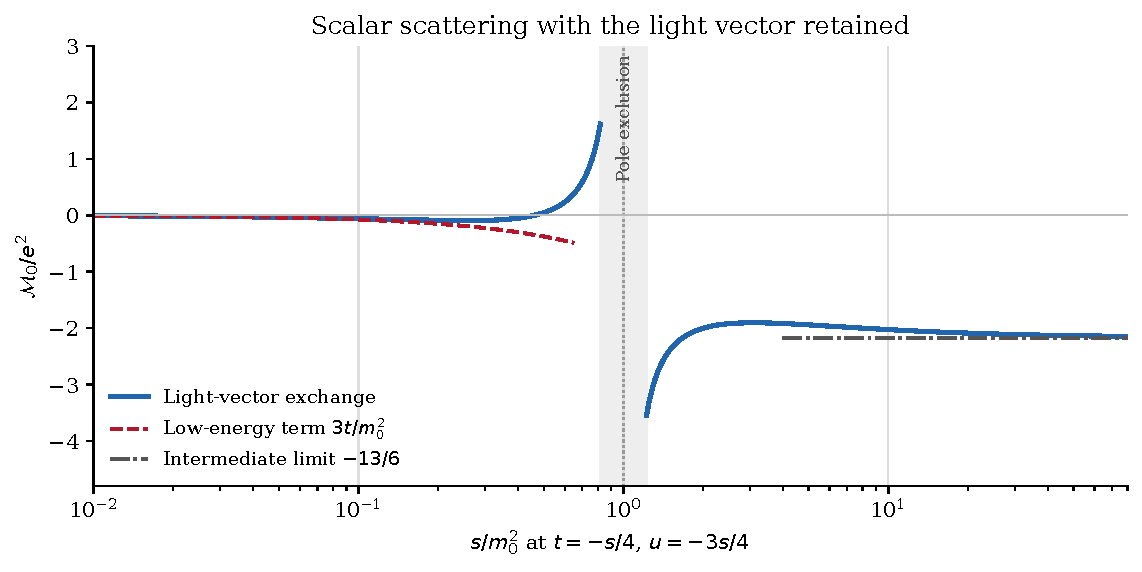
\includegraphics[width=.94\textwidth]{figures/output/threshold_amplitude.pdf}
\caption{The explicit amplitude \eqref{eq:modelamplitude} at fixed angle,
with $b/a=0.1$, $\theta_H=0.8$ and $\delta=0.1$. The shaded interval
is excluded by the light-pole separation. The low-energy curvature term
and the intermediate limit describe different parts of the allowed
window. These are analytic finite-model curves; the actual amplitude
is compared with them by Theorem~\ref{thm:amplitude}, whose error
constant is not numerically evaluated.}\label{fig:threshold}
\end{figure}

\subsection{Uniform curvature of the selected plane}
There is also a geometric consequence of the same vertices. In real
unitary $L^2$ normalization the quotient curvature is
\begin{equation}\label{eq:spectralcurvature}
 K_{\mathbb R}=\sum_{n>0}\frac1{\mu_n}
 \left[3j_n^2+\sum_{\alpha=1}^3
 \left\{b_{n\alpha}(\mathsf u,\mathsf u)b_{n\alpha}(\mathsf v,\mathsf v)
              -b_{n\alpha}(\mathsf u,\mathsf v)^2\right\}\right].
\end{equation}
Indeed twice differentiating the moment equations gives second
fundamental form component $-b_{n\alpha}(w,z)/\sqrt{\mu_n}$ in
the normal direction $n_{n\alpha}$. The Gauss equation gives the
terms involving $b$. Differentiating the mechanical gauge connection
gives O'Neill's contribution $3\sum_n j_n^2/\mu_n$
\cite{oneill,bielawski,bielawski_erratum}.

This calculation applies at each fixed $b>0$ in a Sobolev slice of
the stable determinant-fixed $E$ block. Remove its ineffective
constant center. The gauge and moment-normal operators then have
bounded elliptic inverses at that point, defining the projections,
second fundamental form and $L^2$ Levi-Civita connection. Neutrality
removes the central cokernel; all other orthogonal-adjoint blocks
have zero vertices on this plane. The complete sums converge by the
fixed complementary gap and \eqref{eq:parsevalvertices}. Thus the
formula does not require a lower bound uniform in $b/a$ on the size
of that local slice.

\begin{proposition}\label{prop:uniformcurvature}
The sectional curvature of the actual harmonic bundle-moduli metric on the transported plane
\eqref{eq:plane}, with positive sign on a sphere, satisfies
\begin{equation}\label{eq:uniformcurvature}
 K_{\mathbb R}=\frac3{4b^2}[1+O(r^2)],\qquad
 K_{\gKS}=\frac3{2b^2}[1+O(r^2)],
\end{equation}
uniformly on \eqref{eq:hierarchycone}.
\end{proposition}
\begin{proof}
The light vector term in \eqref{eq:spectralcurvature} is
$3/(4b^2)[1+O(r^2)]$. The light normal terms are $O(r^4/b^2)$,
the other low terms are $O(r^4/a^2)$, and the complementary sum is
$O(1)$. Relative to $1/b^2$, each error is $O(r^2)$ or smaller.
The real unitary metric is twice the Dolbeault metric, so
$K_{\gKS}=2K_{\mathbb R}$.
\end{proof}

This result concerns the specified plane. It asserts neither bounded
derivatives of the full quotient metric nor uniform curvature control
on every plane. Appendix~\ref{sec:derivatives} gives a complementary
regular-patch derivative argument and an explicit singular horizontal
projector.
